\begin{figure}[h!]
\centering
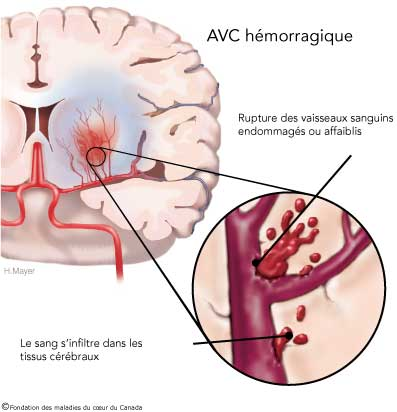
\includegraphics[width=0.5\linewidth]{../images/avc}
\caption{Accident Vasculaire Cérébrale (AVC).}
\end{figure}

Les accidents vasculaires cérébraux (AVC) peuvent être la cause d'hémiplégie chez les personnes qui en sont victimes. La paralysie peut affecter une ou plusieurs parties du corps, jusqu'à être totale si la face, le tronc et les membres supérieurs et inférieurs sont paralysés. \\
La récupération des fonctions motrices, de la parole ou de la compréhension dépendent pour beaucoup de l'âge du patient et de son atteinte au niveau du cerveau.
    \section{Problématique}
Il existe de nombreux tests et échelles pour évaluer les capacités sensorimotrices de patients hémiplégiques \footnote{voir l'Analyse de la littérature \textit{Evaluation of the disabilities of hemiplegic patients [M.-C. Gellez-Leman et al.]}}. Cependant, les médecins se retrouvent souvent confrontés au problème de la précision des mesures lors des test. Si la question ne se pose pas pour les tests dits \textit{fonctionnels} (ex : le patient arrive t-il à se servir un verre d'eau?), des mesures d'angles et de positions se révèlent souvent nécessaires pour valider ou non la réussite d'un test par le patient.
\\Or, il existe peu d'outils pour réaliser ces mesures, et ceux-ci ne font pas l'unanimité. Pour la mesure d'angle entre les membres du patient (pli de l'épaule, du coude, etc.), le goniomètre se révèle être l'outil le plus utilisé, mais probablement par défaut (cf \ref{lapeyronie} ). On lui reprochera en effet d'être: 
\begin{itemize}
  \item {intrusif :} Il doit être en contact direct avec le patient, pouvant fausser la mesure ou aider/gêner le patient.
  \item {imprécis :} L'épaisseur de peau et de graisse ne permet pas d'évaluer correctement l'angle formé par les os.
  \item {inutilisé :} Des médecins pourtant équipés vont préférer juger à l'œil, pour un meilleur ratio temps/précision.
\end{itemize}

    \subsubsection{Le test de Fugl-Meyer}
Cette imprécision des mesures devient dès lors gênante lorsque c'est un test non pas fonctionnel, mais de déficience qui est considéré comme le "Gold Standard" dans le domaine : le score de Fugl Meyer [\ref{fugl_meyer}]. En effet, celui-ci consiste à évaluer les mouvements du patient lors de la réalisation de gestes très précis, incluant des mouvements "éliminatoires", qu'il faut donc être capable de mesurer.  
  
  L'idée s'est alors posée d'utiliser un autre moyen de mesure, moins intrusif, pour la réalisation du test de Fugl Meyer, largement utilisé dans le milieu de la réhabilitation, et de réfléchir aux possibilités d'enrichissement de celui-ci.
\newpage
    \section{Présentation du projet}
    
      \subsection{Étude de terrain} \label{etude_terrain}
    Le projet est avant tout une étude de faisabilité. Nous essayerons de voir
    à quel point nous pouvions procéder, avec un capteur de profondeur (en
    l'occurrence la Microsoft Kinect) et des bibliothèques et outils couramment 
    disponibles, à un test complet ou partiel de Fugl-Meyer.
    
    Nous étudierons donc d'une part les technologies disponibles pour la Kinect,
    et d'autre ce qu'est le test de Fugl-Meyer et quelles sont les 
    problématiques associées.
    
    \subsection{Prototype}
    Nous élaborerons ensuite une preuve de concept, c'est à dire un 
    prototype proposant au patient en cours de réhabilitation un test partiel 
    de Fugl-Meyer. Les points importants à considérer pour un tel prototype 
    sont~:
    \subsubsection{Automatisation et objectivité}
    Le système doit pouvoir procéder à une évaluation, de manière non-intrusive 
    et sans intervention externe, de ce qui se trouve devant lui. Il doit donc 
    proposer une série de notes objectives qui correspondent aux performances du 
    patient.
    \subsubsection{Aspect ludique~: "gamification"}
    La "gamification" est le processus qui consiste à ajouter des éléments 
    souvent associés au domaine du jeu (d'où le nom), comme des barres de
    progression ou des défis à relever, à une activité non-ludique. L'idée est 
    de favoriser l'implication et la motivation des participants. 
    Notons qu'il ne s'agit pas nécessairement de faire de l'activité en soi un 
    jeu.
    \subsubsection{Retour d'information continue et granulaire}
    La "granularité" d'un retour est le nombre d'options possibles. 
    Chaque exercice du Fugl-Meyer, par exemple, est noté sur trois points 
    (0, 1 ou 2). Nous 
    aimerions proposer une alternative plus nuancée.
    L'argument pour le retour d'information rejoint celui de la "gamification"~:
    la notion de "sens" dans un jeu, au moins d'après Salen et 
    Zimmerman\cite{rules_of_play}, est 
    directement liée à la richesse de ce retour.
